\documentclass[letter]{article}
\usepackage{amsmath}
\usepackage{amsfonts}
\usepackage{amssymb}
\usepackage{bm}
\usepackage{ifthen}
\usepackage{fancyhdr}
\usepackage{graphicx}
\usepackage[hidelinks]{hyperref}
\usepackage{xcolor}
\hypersetup{
    colorlinks,
    linkcolor={red!50!black},
    citecolor={blue!50!black},
    urlcolor={blue!80!black}
}

\definecolor{deepblue}{rgb}{0,0,0.5}
\definecolor{deepred}{rgb}{0.6,0,0}
\definecolor{deepgreen}{rgb}{0,0.5,0}

\usepackage{listings}
\usepackage{tkz-graph}
\usetikzlibrary{arrows}

% Default fixed font does not support bold face
\DeclareFixedFont{\ttb}{T1}{txtt}{bx}{n}{12} % for bold
\DeclareFixedFont{\ttm}{T1}{txtt}{m}{n}{12}  % for normal

% Python style for highlighting
\newcommand\pythonstyle{\lstset{
language=Python,
basicstyle=\ttm,
otherkeywords={self},             % Add keywords here
keywordstyle=\ttb\color{deepblue},
emph={MyClass,__init__},          % Custom highlighting
emphstyle=\ttb\color{deepred},    % Custom highlighting style
stringstyle=\color{deepgreen},
frame=tb,                         % Any extra options here
showstringspaces=false            % 
}}


% Python environment
\lstnewenvironment{python}[1][]
{
\pythonstyle
\lstset{#1}
}
{}

% Python for external files
\newcommand\pythonexternal[2][]{{
\pythonstyle
\lstinputlisting[#1]{#2}}}

% Python for inline
\newcommand\pythoninline[1]{{\pythonstyle\lstinline!#1!}}


%%%
% Set up the margins to use a fairly large area of the page
%%%
\oddsidemargin=.2in
\evensidemargin=.2in
\textwidth=6in
\topmargin=-.5in
\textheight=9in
\parskip=.07in
\parindent=0in
\pagestyle{fancy}

%%%
% Set up the header
%%%
\newcommand{\setheader}[6]{
	\lhead{{\sc #1}\\{\sc #2} ({\small \it \today})}
	\rhead{
		{\bf #3} 
		\ifthenelse{\equal{#4}{}}{}{(#4)}\\
		{\bf #5} 
		\ifthenelse{\equal{#6}{}}{}{(#6)}%
	}
}

\makeatletter
\newcommand{\escapeus}{\begingroup\@makeother\_\@escapeus}
\newcommand*{\@escapeus}[1]{#1\endgroup}
\makeatother

%%%
% Set up some shortcut commands
%%%
\newcommand{\R}{\mathbb{R}}
\newcommand{\N}{\mathbb{N}}
\newcommand{\Z}{\mathbb{Z}}
\newcommand{\C}{\mathbb{C}}
\newcommand{\Proj}{\mathrm{proj}}
\newcommand{\Perp}{\mathrm{perp}}
\newcommand{\proj}{\mathrm{proj}}
\newcommand{\Span}{\mathrm{span}}
\newcommand{\Null}{\mathrm{null}}
\newcommand{\Rank}{\mathrm{rank}}
\newcommand{\mat}[1]{\begin{bmatrix}#1\end{bmatrix}}
\newcommand{\var}[1]{{$\langle$\it #1$\rangle$}}
\newcommand{\Code}[1]{\texttt{\escapeus #1}}
\DeclareMathOperator{\Tr}{Tr}

%%%
% This is where the body of the document goes
%%%
\begin{document}
	\setheader{MAT335}{Homework 4}{Due: 11:59pm April 6}{}{}{}

	\begin{enumerate}
		\item For a dynamical system $(T,X)$, a point $x\in X$ is called \emph{eventually periodic} if there 
			exists $m>m'$ so that $T^mx=T^{m'}x$.
		\begin{enumerate}
			\item Let $(T,[0,1))$ be the doubling map and let $(\sigma,\Omega)$ be the full two shift.
				For each system, give an example of (i) a point that is eventually periodic, and (ii)
				a point that is eventually periodic but \emph{not} periodic.
			\item Let $\C$ be the coding function for the doubling map with the usual partition ($\mathcal P_0=[0,1/2)$
				and $\mathcal P_1=[1/2,1)$).

				Prove $\C(x)$ is eventually periodic in $(\sigma, \Omega)$ if and only if $x$ is eventually
				periodic in $(T,[0,1))$.
			\item Prove that $\C(x)$ is eventually periodic if and only if $x$ is a rational number.
			\item Prove that a binary expansion of a number in $[0,1)$ is eventually periodic if and only
				if that number is rational. (\emph{Hint: $\C(x)$ is always a binary expansion, but not all
				binary expansions come from codings}).
			\item Prove that the base $n$ expansion of a number in $[0,1)$ is eventually periodic if an only if that
				number is rational.
		\end{enumerate}

		\item Let $(\sigma, \Omega)$ be the full two-shift. Let $G\subseteq\Omega$ 
			bet the set of sequences without two ones in a row.
			Let $X\subseteq \Omega$ be the set of sequences without \emph{three} ones in a row.
			\begin{enumerate}
				\item Show that $(\sigma, X)$ is a subshift.
				\item A \emph{two-step} Markov chain is a Markov chain where the transition probabilities
					between states depend on the current state \emph{and} the previous state. 
					
					A \emph{two-step} Markov chain on a state space $S$ can be thought of as a 
					one-step (regular) Markov chain on the state space $S\times S$. For example, let
					$\mathcal M$ be the Markov
					chain on states $0$ and $1$ with equal transition probabilities.
					Normally, $\mathcal M$ has a graph like this:

					\begin{center}
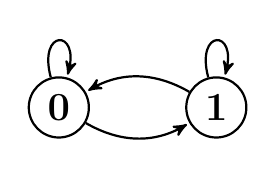
\begin{tikzpicture}[->,>=stealth',shorten >=1pt,auto,node distance=2cm,
                thick,main node/.style={circle,draw,font=\Large\bfseries}]
  \node[main node] (1) {0};
  \node[main node] (2) [right of=1] {1};


  \path
    (2) edge [loop above] (2);

  \path
    (1) edge [loop above] (1)
	edge [bend right] (2)
    (2) edge [bend right] (1)
    ; 
\end{tikzpicture} 
					\end{center}

	However, we can also model $\mathcal M$ as a Markov chain $\mathcal M'$
					with state space $00$, $01$, $10$, and $11$ and transition graph like this:
					\begin{center}
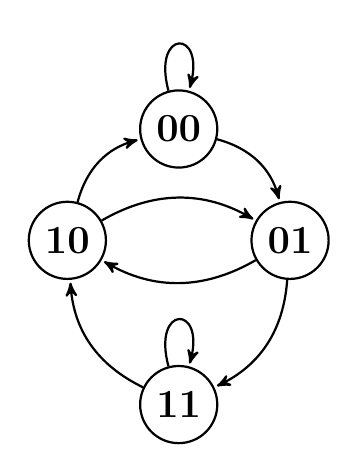
\begin{tikzpicture}[->,>=stealth',shorten >=1pt,auto,node distance=2cm,
                thick,main node/.style={circle,draw,font=\Large\bfseries}]
  \node[main node] (00) {00};
  \node[main node, yshift=-1.5cm] (11) [below of=00] {11};
  \node[main node] (01) [below right of=00] {01};
  \node[main node] (10) [below left of=00] {10};


  \path
    (11) edge [loop above] (11);

  \path
    (00) edge [loop above] (00);

  \path
    (11) edge [bend left] (10)
    (01) edge [bend left] (10)
    (01) edge [bend left] (11)
    (10) edge [bend left] (00)
    (10) edge [bend left] (01)
    (00) edge [bend left] (01)
    ; 
\end{tikzpicture} 

					\end{center}
		Explain how $\mathcal M'$ models $\mathcal M$. In particular, explain why the graph for $\mathcal M'$ has no edge between $00$ and $11$.

		\item Let $\mathcal M_G$ be a Markov chain whose set of realizations is $G$.
			\begin{enumerate}
				\item Draw a graph for $\mathcal M_G$ and find its associated transition matrix.
				\item Use the transition matrix for $\mathcal M_G$ to compute the entropy of $(\sigma, G)$.
				\item Model $\mathcal M_G$ as a two-step Markov chain  $\mathcal M_G'$, which can be viewed as a Markov chain
					with state space $\{00,01,10,11\}$. 

					Draw the graph associated with $\mathcal M_G'$ and find its transition matrix.
				\item Using the transition matrix for $\mathcal M_G'$, compute the entropy of $(\sigma, G)$.
			\end{enumerate}
		\item Can $X$ be modeled by a one-step Markov chain? Why or why not?
		\item Find the entropy of $(\sigma, X)$.
			\end{enumerate}

		\item Let $(\sigma, \Omega)$ be the full two shift.
		\begin{enumerate}
			\item Prove that $(\sigma, \Omega)$ is \emph{expansive}.
			\item Prove that $(\sigma, \Omega)$ is \emph{transitive}.
			\item Show that $(\sigma, \Omega)$ is \emph{chaotic}.
			\item Let $(T,X)$ be a dynamical system and let $x,y\in X$. We say $x$ and $y$ are
				\emph{$\delta$-correlated for $n$ steps} if the distance between $T^ix$ and $T^iy$ is
				at most $\delta$ for $i=0,\ldots, n$.

				Let $x,y\in \Omega$ be points that are at distance $2^{-k}$ of each other. For how many steps will
				$x$ and $y$ be $\delta$-correlated when $\delta=1/4$?
			\item If $(T,X)$ is a chaotic dynamical system, can two points be $\delta$-correlated indefinitely? What implications
				does this have for measurement error?
		\end{enumerate}


	\item Two dynamical systems $(T, X)$ and $(S,Y)$ are called \emph{conjugate} if there exists a continuous, invertible
		function $\Phi:Y\to X$ so that $T=\Phi^{-1}\circ S\circ \Phi$. In this case, $\Phi$ is called a \emph{conjugacy}.

		The systems are called \emph{semi-conjugate} if there
			exist continuous, onto function $\Phi:Y\to X$ so that
			$T\circ\Phi$ = $\Phi\circ S$. In this case, $\Phi$ is called a \emph{semi-conjugacy}.


		\begin{enumerate}
			\item Let $(T,X)$ and $(S,Y)$ be conjugate dynamical systems.
				\begin{enumerate}
					\item Show that if there exists a point of period $k$ in $Y$, there exists a point
						of period $k$ in $X$.
					\item Show that if $(S,Y)$ is transitive, then $(T,X)$ is transitive.
					\item Is it true that if $(S,Y)$ is expansive, then $(T,X)$ is necessarily expansive?
				\end{enumerate}
			\item Prove that if $(T,X)$ and $(S,Y)$ are conjugate dynamical systems, that they are also semi-conjugate dynamical
				systems.
			\item Let $(T,X)$ and $(S,Y)$ be semi-conjugate dynamical systems.
				\begin{enumerate}
					\item Show that if there exists a point of period $k$ in $Y$, there exists a point
						of period $\leq k$ in $X$.
					\item Show that if $(S,Y)$ is transitive, then $(T,X)$ is transitive.
					\item Is it true that if $(S,Y)$ is expansive, then $(T,X)$ is necessarily expansive?
				\end{enumerate}
			\item Let $(T,[0,1))$ be the doubling map and let $(\sigma, \Omega)$ be the full two shift.
				\begin{enumerate}
					\item Show that $(T,[0,1))$ and $(\sigma, \Omega)$ are semi-conjugate.
					\item Show that $(T,[0,1))$ is chaotic.
				\end{enumerate}
			\item Let $(T,[0,1))$ be the doubling map and let $(L,[0,1))$ be the \emph{logistic map} defined by
				$L(x)=rx(1-x)$ for $r=4$.
				\begin{enumerate}
					\item Define $f:[0,1)\to[0,1)$ by $f(x)=\sin^2(2\pi x)$. Show that $f$ is a semi-conjugacy
						between $(L,[0,1))$ and $(T,[0,1))$.
					\item Show that $(L,[0,1))$ contains points of every period.
					\item Show that $(L,[0,1))$ is chaotic.
				\end{enumerate}
		\end{enumerate}

	\end{enumerate}


	\subsection*{Programming Problems}
	For the programming problems, please use the Jupyter notebook available at

	\url{https://utoronto.syzygy.ca/jupyter/user-redirect/git-pull?repo=https://github.com/siefkenj/2020-MAT-335-webpage&subPath=homework/homework4-exercises.ipynb}

	Make sure to comment your code and use ``Markdown'' style cells to explain your answers.

	\begin{enumerate}
		\item The \emph{logistic map with parameter $r$} is the function $f:[0,1]\to[0,1]$ defined by $f(x)=rx(1-x)$ (for $r\in[0,4]$).
			It was invented as a simple model for population in biology. The idea is that if $x$ is your original population,
			there will be some birth rate $r$ governing population growth; however, when the population outstretches its
			resources, its growth will be constrained. The $1-x$ parameter models this constraint on growth.

			Despite being so simple, the logistic map can have amazingly complex behaviour!

		\begin{enumerate}
			\item A two-parameter logistic function {\tt f} has been predefined. Create a function \verb|orbit_f| which inputs
				a starting value, a parameter $r$, and an orbit length $n$, and returns a list with the first
				$n$ points along the orbit of {\tt f}.

			\item \label{PARTIALORBIT}Given a dynamical system $(T,X)$, the $n$-orbit of $x$ is $\mathcal O^n(x)=\{x,Tx,\ldots, T^{n-1}x\}$.

				Using $r=2$, plot the 20-orbits of $x$ for at least 10 different $x$'s (plot time vs.~value). What do you notice?
			\item Does the logistic map with $r=2$ have a \emph{basin of attraction}\footnote{ Look back in the notes
				if you've forgotten this term.}? Justify your conclusion.
			\item Repeat part \ref{PARTIALORBIT} using $r=3$. What do you notice? Is there a basin of attraction consisting of a single point?

			\item In general, a \emph{basin of attraction} for a dynamical system is a set which all points limit to.
				Does the logistic map have a basin of attraction when $r=3$? If so, describe it.

			\item Repeat part \ref{PARTIALORBIT} with $r=4$. Is there a basin of attraction? Why or why not?
		\end{enumerate}

		\item We are going to plot the basins of attraction for the logistic map as a function of $r$. We can approximate a basin
			of attraction by taking the $1000$-orbit of several points, and then taking the set consisting of the last $100$ points
			in each orbit.

		\begin{enumerate}
			\item Create a function \verb|approximate_basin| which takes in a parameter $r$ and returns a list
				of points that approximate the basin of attraction of the logistic map with parameter $r$.

				\emph{Hint:} It may be useful to round your results to 3 or 4 decimal places and then use {\tt np.unique}
				to get a list of manageable length.
			\item Plot the basins of attraction of the logistic map vs.~$r$ for at 1000 different values of $r$ between $0$
				and $4$.
			\item What do you notice about the basins of attraction? Did you expect this?
			\item In the \emph{proofs} part of this homework set, you proved that the logistic map is chaotic when $r=4$.
				What does that imply about the basin of attraction?

			\item If a population is well-modeled by the logistic map with a parameter of $r=3.82$, what can you say about the population
				after 1000 days? What if it is modeled by a logistic map with parameter $r=3.83$? Is the population more or less
				predictable?
		\end{enumerate}

	\end{enumerate}



\end{document}
